\documentclass[ncrna,article,submit,moreauthors,pdftex,10pt,a4paper]{mdpi}

\usepackage{color}
\usepackage[utf8]{inputenc}

\Title{Supplementary File 2}
\Author{}
\address{}

\begin{document}

In order to investigate the influence of the dataset size on the complexity of gene structures, we calculated the average number of introns for a series of different dataset sizes.
Therefore, we used RNA-Seq data from 111 lymphoma samples  consisting of the different subtypes BL, FL and DLBCL that was published in the context of the ICGC MMML-Seq project \citep{Richter2012-un}.
After mapping the reads onto the human reference genome using the splice-aware mapping tool \textit{segemehl} \citep{hoffmann2009, hoffmann2014}, read support for all the identified splice junctions, i.e. genomic interval spanning exon-exon boundaries, were calculated. After applying a certain minimum read support filter of 1, 5 and 10, the average intron number per annotation item was computed. This procedure was performed using all dataset sizes from one sample to all 111 samples (Fig. \ref{saturation}).

\begin{figure}[H]
 \centering
 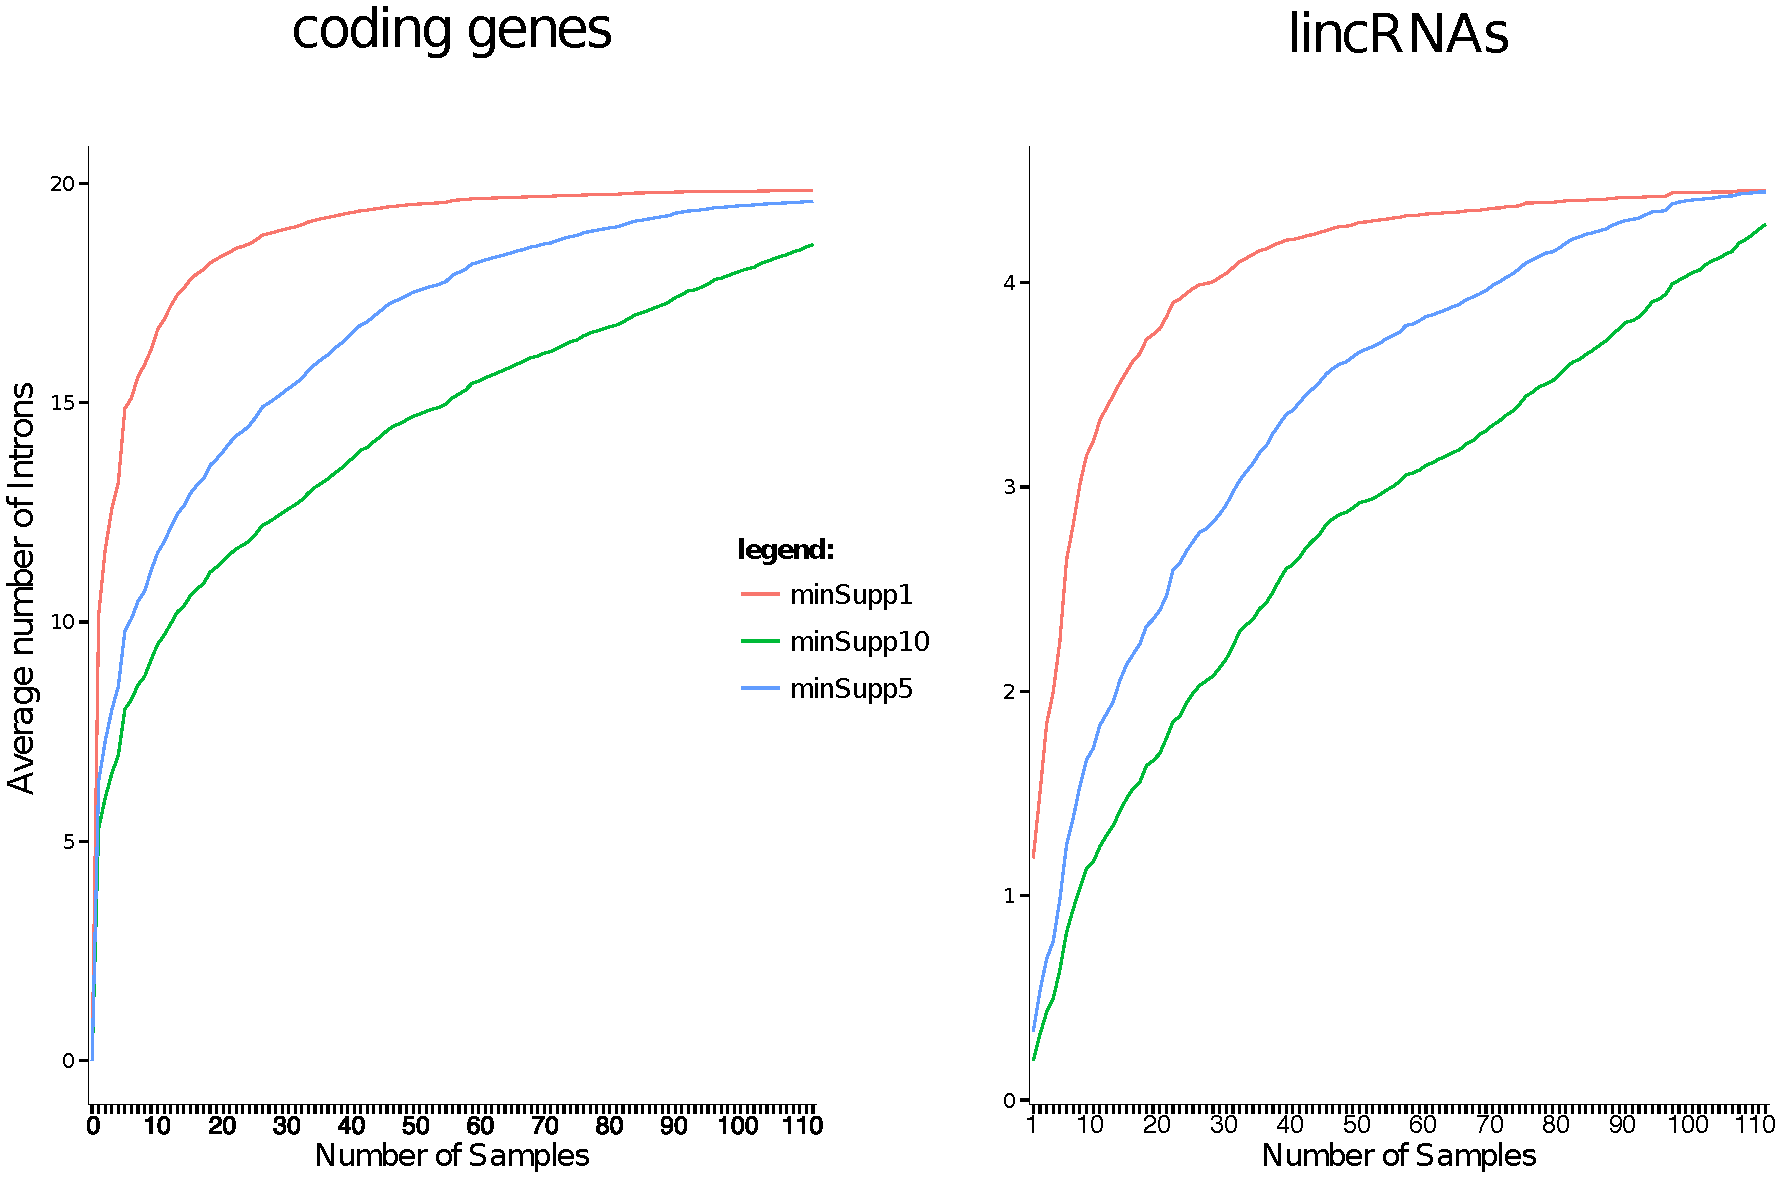
\includegraphics[width=\linewidth]{saturation}
 \caption{
Average number of introns per gene based on different data set sizes (on the left for coding genes on the right for lincRNAs). Three different minimum read support thresholds are displayed.
For both classes (coding genes and lincRNAs) the complexity of the gene structure increases by considering more data. However, a saturation of this trend is observable (19.2 for the coding genes and 4.3 for the lincRNAs). Obviously, this saturation in complexity increase is more prominent for the smallest thresholds of minimum read support.}
 \label{saturation}
\end{figure}

Based on the complete data set of all 111 samples we divided the genes according to their normalized mean expressions (RPKM) and counted for all expression bins the number of genes for that we computed more, less or an equal number of introns compared to the annotation using a minimum read support of 10 (Fig. \ref{scatter}). 

\begin{figure}[h]
 \centering
 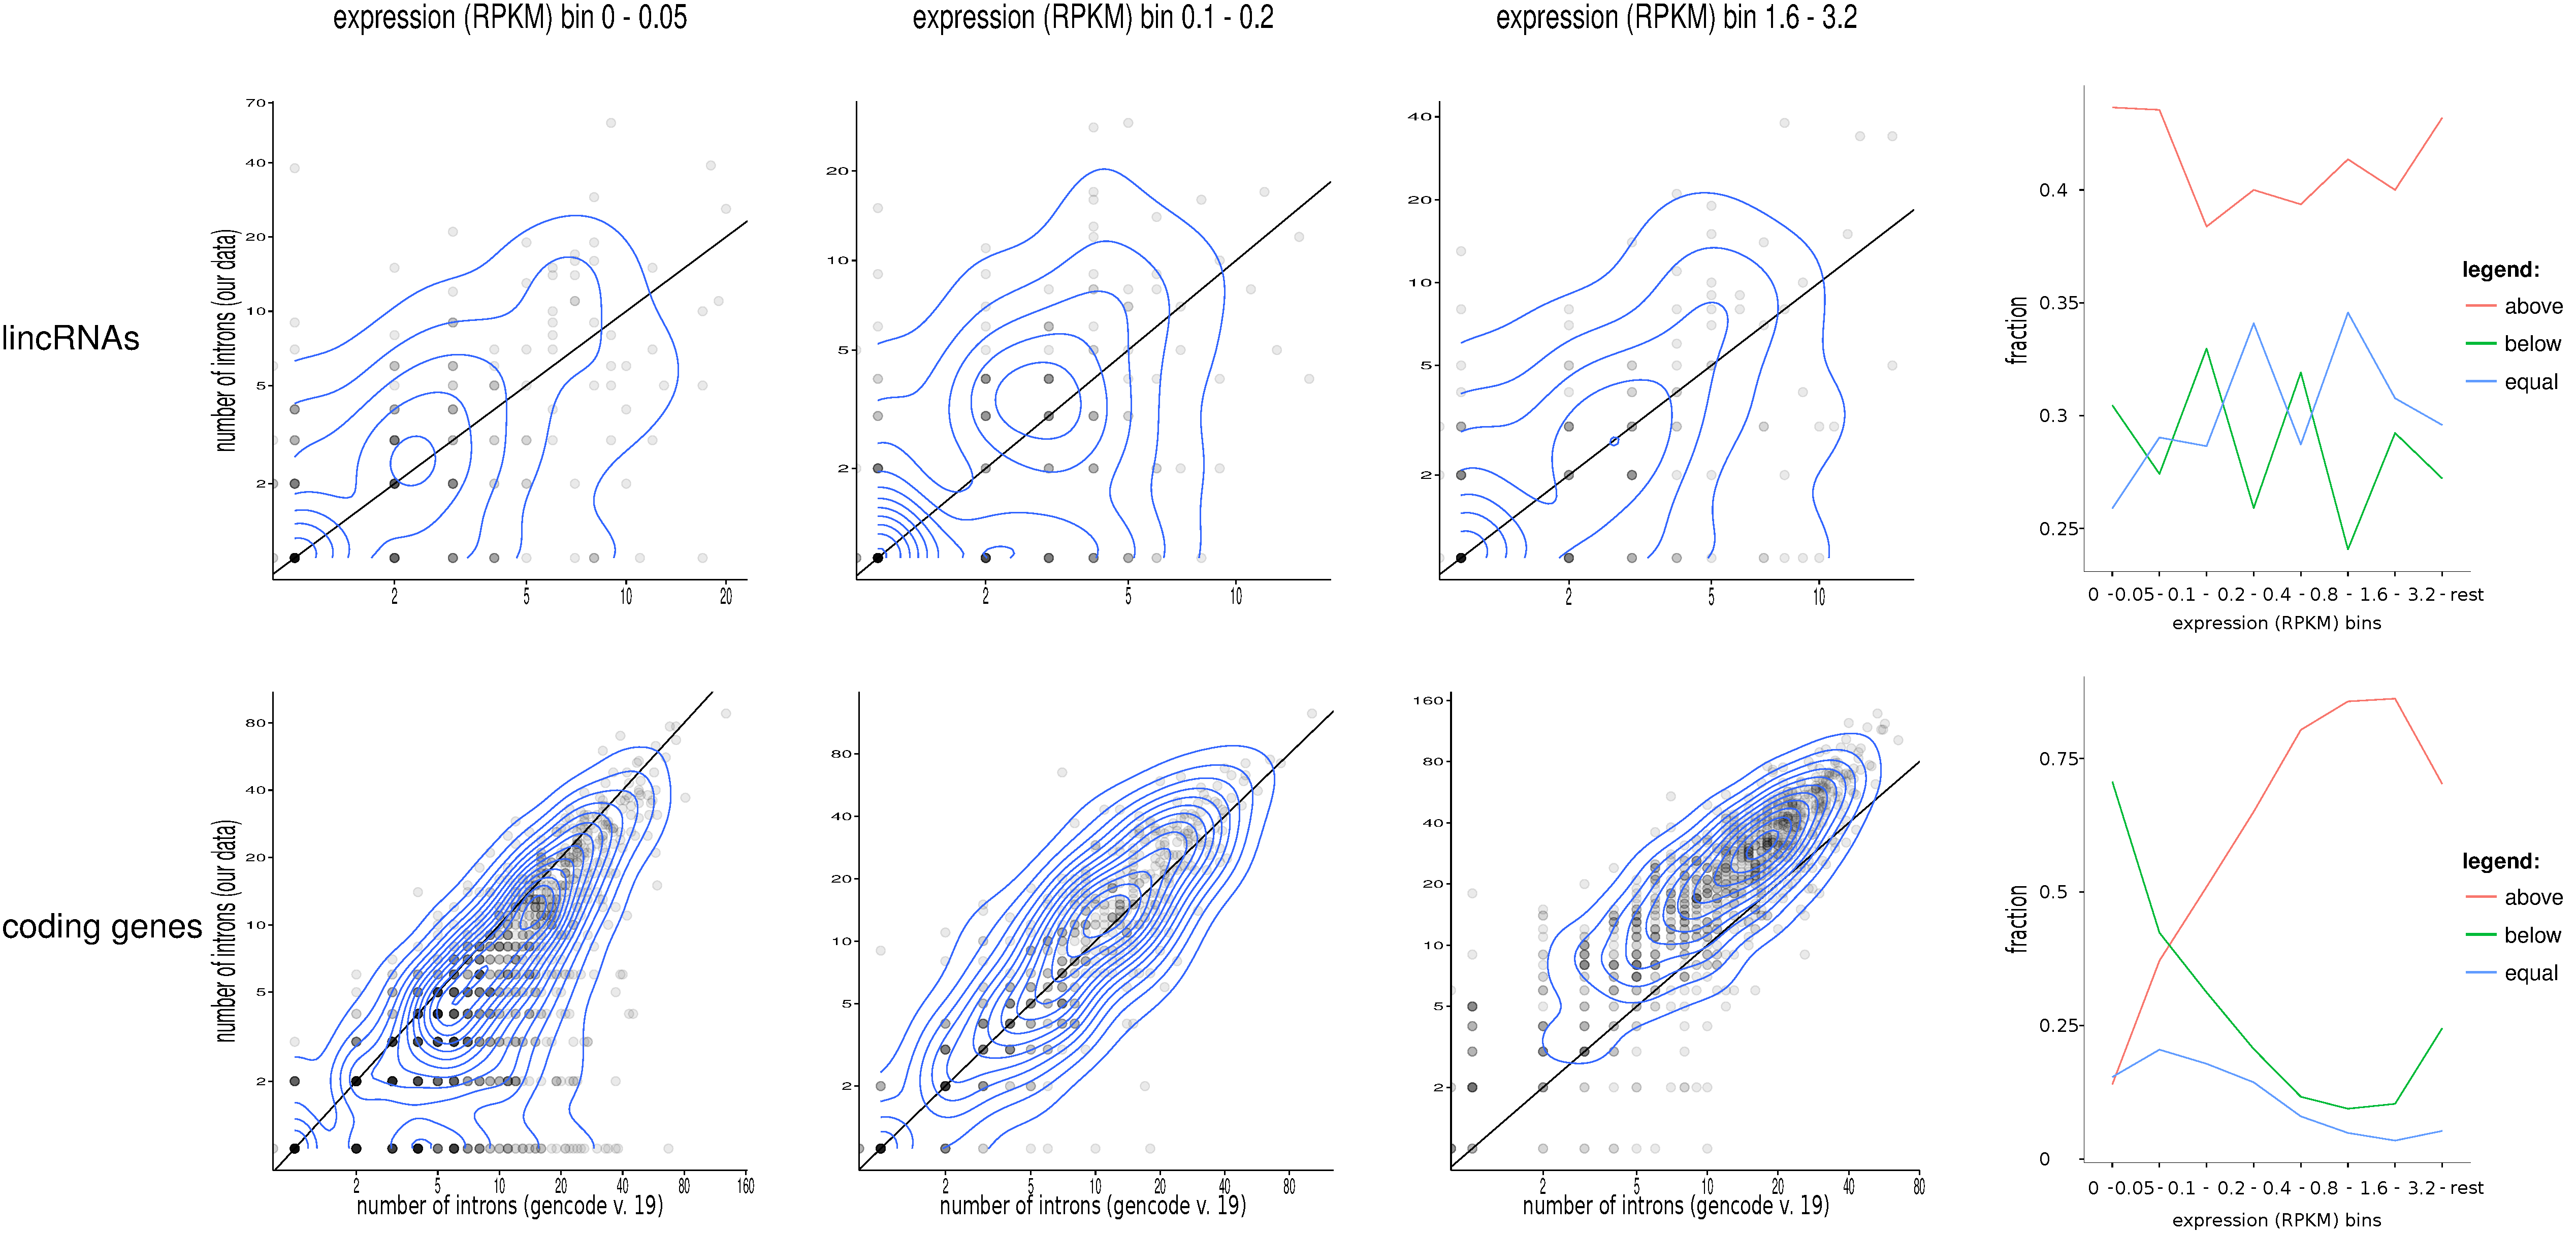
\includegraphics[height = 10 cm, width=\linewidth]{Fig1.pdf}
 \caption{Scatterplots for different number of expression bins for lincRNAs and coding genes. 
The diagonal is the X=Y line. Points above the line are those genes for that we calculate more introns compared to GENCODE v19.
The right most column shows the fraction of genes being above, below and on the line  in relation to the expression.
While for the coding genes a clear shift of these fractions over the different expression bins is visible, we observe for all expression bins more genes for that we predict more introns compared to the GENCODE v19 annotation.}
 \label{scatter}
\end{figure}

Fig. \ref{comparison} shows the distribution of introns per gene between the dataset and GENCODE v19. We compared the number of introns of every gene from the dataset as we calculated with the same genes as found in GENCODE. Although a similarity could be noticed, we computed a number of genes to have higher number of introns than in GENCODE.
\clearpage
\begin{figure}[h]
 \centering
 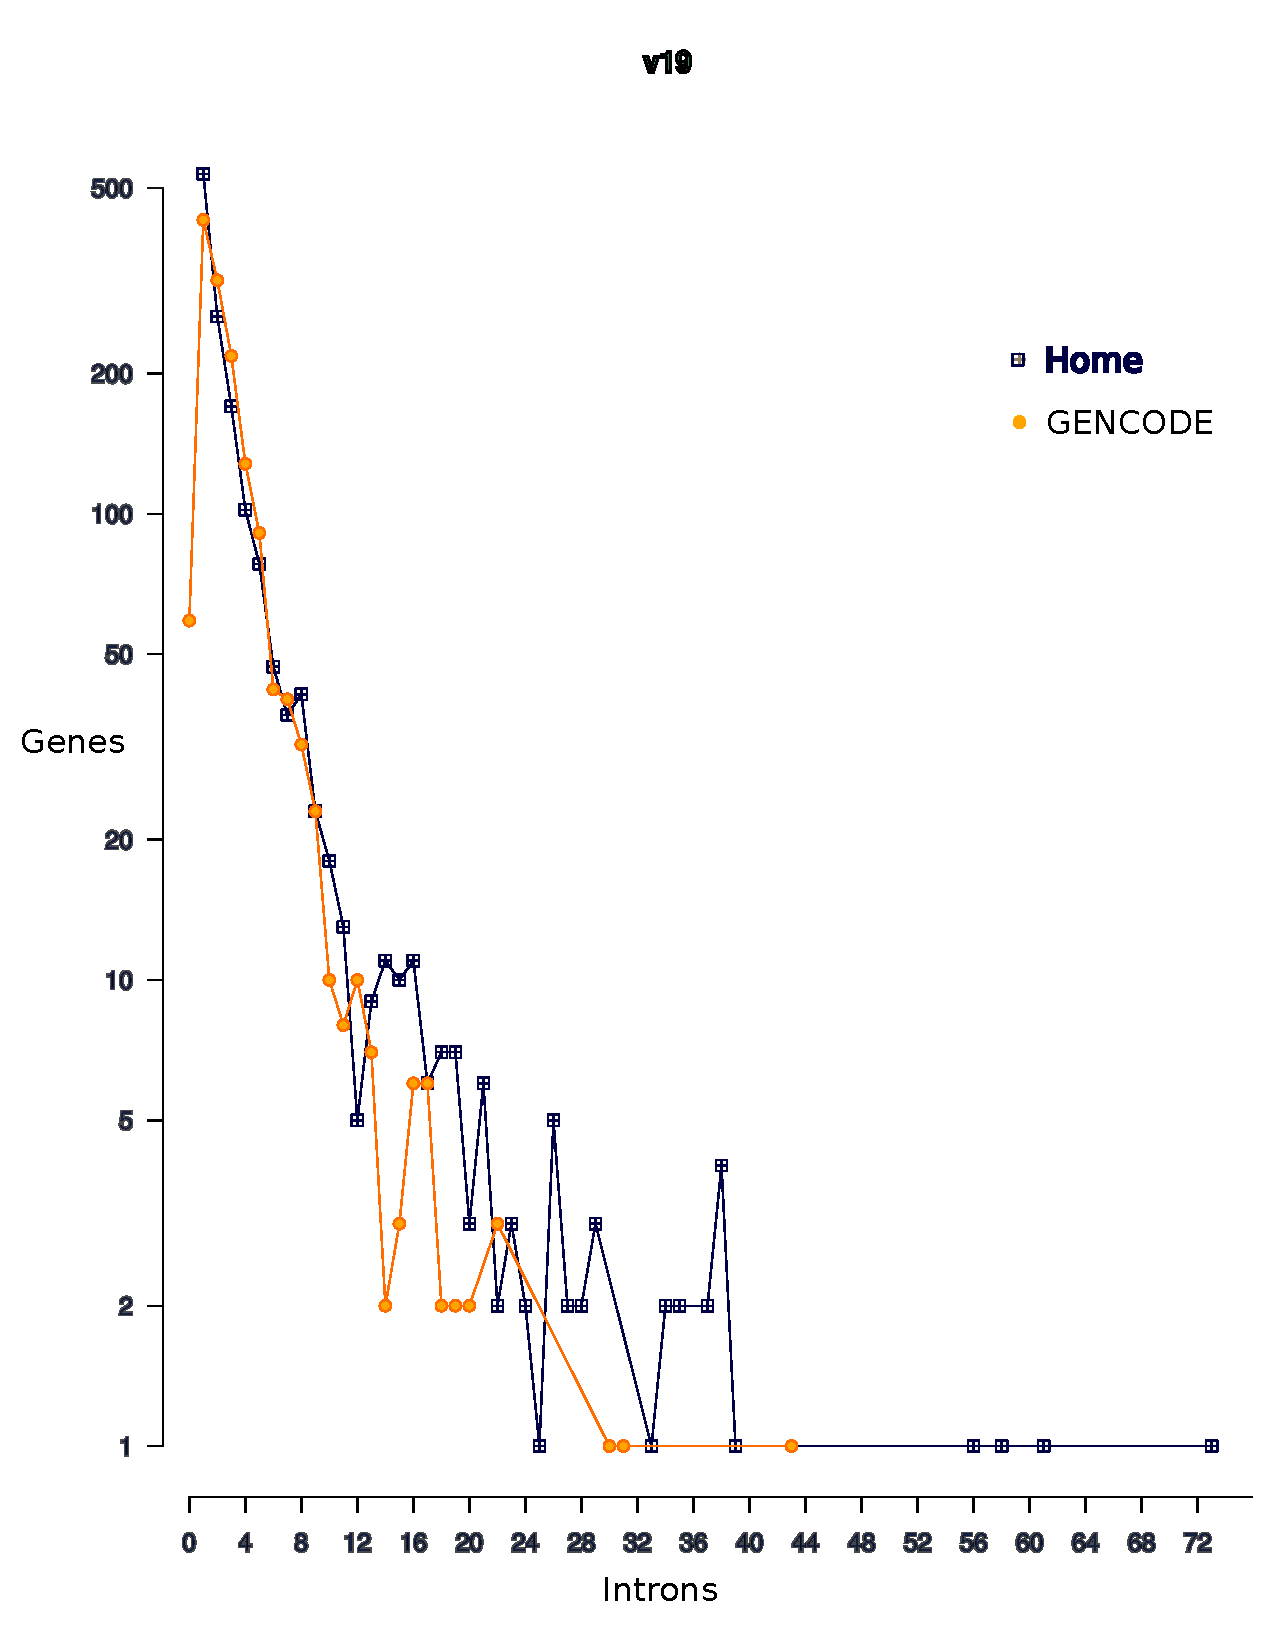
\includegraphics[height = 12 cm, width=14 cm]{comparison_plot_2}
 \caption{The annotations of the lincRNAs from the RNA-Seq data were compared against the annotations of the same lincRNAs found in GENCODE. A considerable number of genes having more introns than reported in GENCODE is shown here.}
 \label{comparison}
\end{figure}

\bibliographystyle{mdpi}
\bibliography{references}

\end{document}
